%affichage dans sommaire sans numero
\chapter{Annexes}
\addcontentsline{toc}{chapter}{Annexes}


\section{Annexe 1 - Triangulation Global/Locale}
\label{AnnexTriangu}
    Dans cette annexe est présentée une expérience complémentaire sur la triangulation globale et locale. MoCapIA utilise la  \textbf{triangulation locale} pour reconstruire les positions 3D des marqueurs. Pour ça le système utilise les coordonnées 3D estimées à partir de chaque paire de caméras, utilise une méthode de \textit{binning} qui consiste à regrouper les points 3D proches dans des \textit{bins} (ou boîtes) de taille fixe, puis on effectue la moyenne du \textit{bins} le plus rempli pour obtenir la position 3D finale du marqueur.

    À première vue, même si on utilise la moyenne, on utilise pour obtenir la triangulation du point 3D seulement deux caméras. Une autre option existe : la \textbf{triangulation globale}. Cette méthode consiste à calculer dans un premier temps les coordonnées 3D à partir d'une paire de caméras, puis de re-projeter ces coordonnées 3D en 2D pour les comparer avec les paramètres 2D de toutes les autres caméras. Le point 3D est donc ajusté pour minimiser l'erreur de reprojection sur toutes les caméras. Cette méthode permet donc d'utiliser l'information de toutes les caméras pour chaque point 3D.

    Pourtant, cette méthode n'a pas été concluante dans le cadre de MoCapIA. En effet, en testant cette méthode sur les données de calibration, on obtient une erreur de reprojection plus importante (voir figure \ref{fig:triangulation_global_local}).
    \begin{figure}[H]
        \centering
        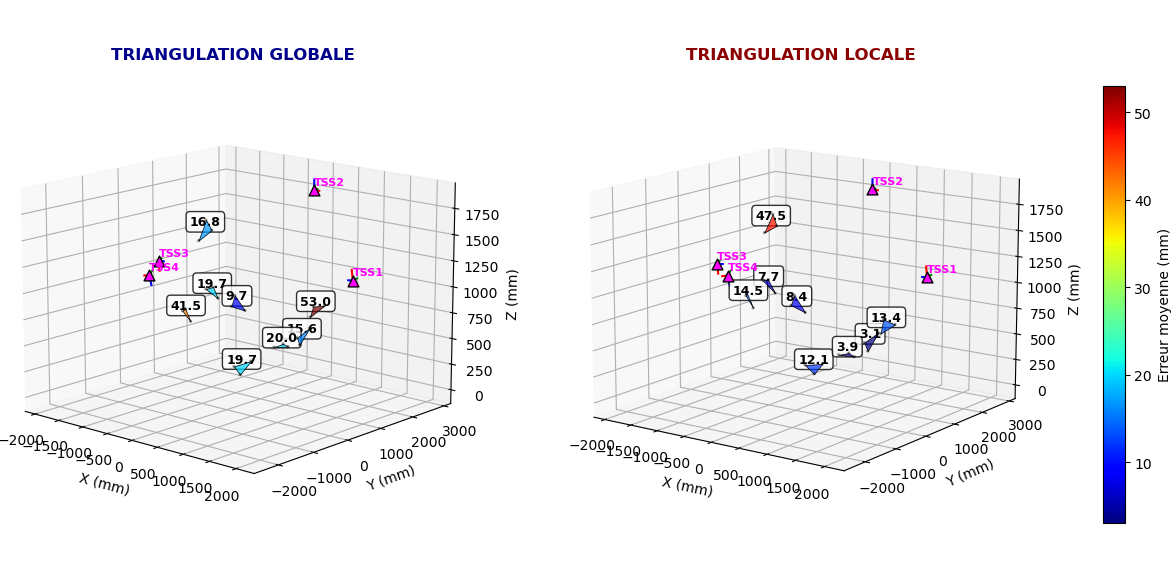
\includegraphics[width=\textwidth]{assets/Capture d'écran process/Précision_CalibTriangulation/triangulation_test.png}
        \caption{Comparaison de l'erreur de triangulation globale et locale}
        \label{fig:triangulation_global_local}
    \end{figure}
    La triangulation locale obtient une erreur moyenne de $13.83mm$ contre $24.50mm$ pour la triangulation globale. On a donc conservé la méthode de triangulation locale pour la suite du stage.

\section{Annexe 2 - Autres résultats de la comparaison Vicon - MoCapIA}
\label{AnnexVicon_Mocap}
    Dans cette annexe sont présentés les résultats complémentaires de la comparaison entre le système de référence Vicon et le système MoCapIA. 

    \begin{figure}[H]
        \centering
        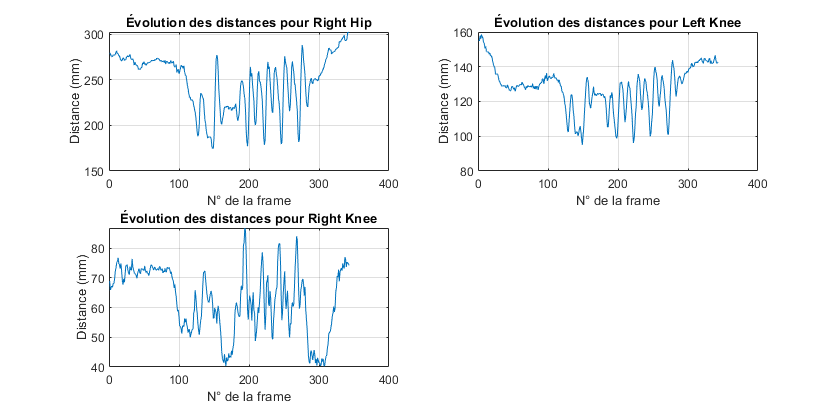
\includegraphics[width=\textwidth]{assets/Capture d'écran process/TX_ViconVSMocapIA/evolution_distance_Mocap.png}
        \caption{Évolution de la distance}
    \end{figure}
    \begin{figure}[H]
        \centering
        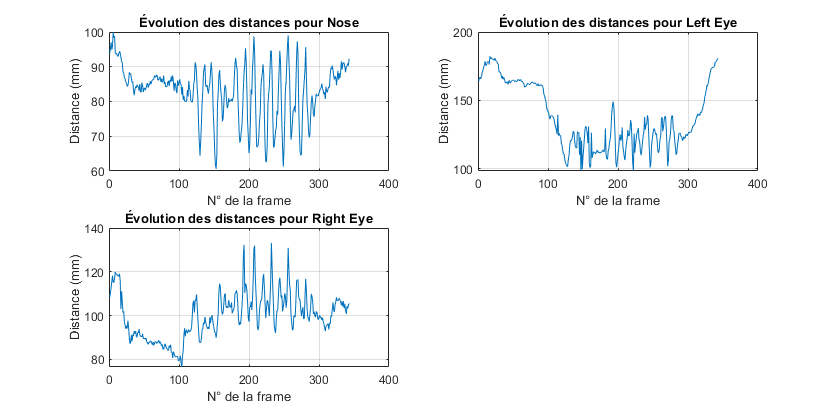
\includegraphics[width=\textwidth]{assets/Capture d'écran process/TX_ViconVSMocapIA/evolution_distance_Mocap11.png}
        \caption{Évolution de la distance}
    \end{figure}
    \begin{figure}[H]
        \centering
        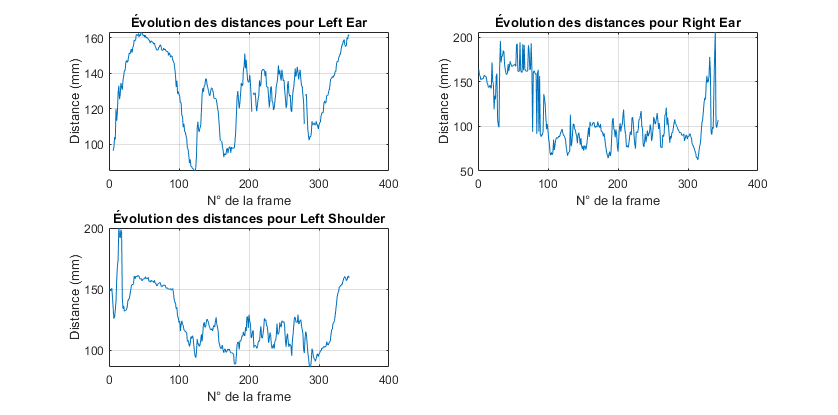
\includegraphics[width=\textwidth]{assets/Capture d'écran process/TX_ViconVSMocapIA/evolution_distance_Mocap12.png}
        \caption{Évolution de la distance}
    \end{figure}
    \begin{figure}[H]
        \centering
        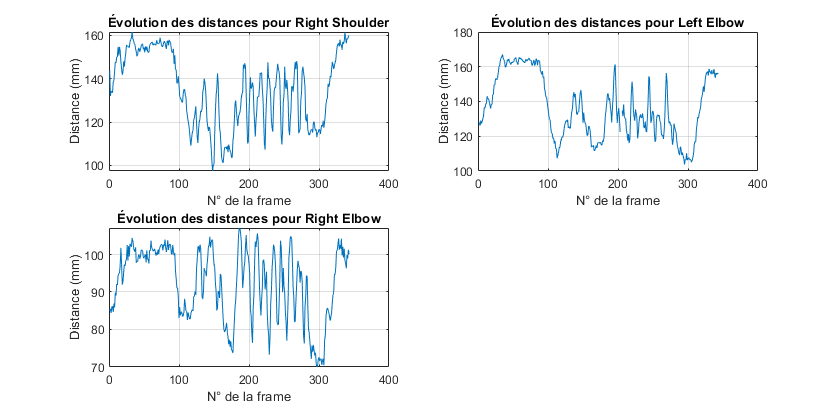
\includegraphics[width=\textwidth]{assets/Capture d'écran process/TX_ViconVSMocapIA/evolution_distance_Mocap13.png}
        \caption{Évolution de la distance}
    \end{figure}
    \begin{figure}[H]
        \centering
        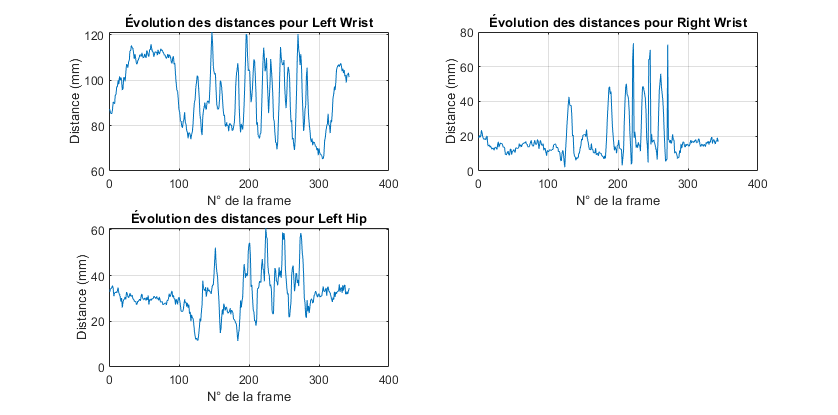
\includegraphics[width=\textwidth]{assets/Capture d'écran process/TX_ViconVSMocapIA/evolution_distance_Mocap14.png}
        \caption{Évolution de la distance}
    \end{figure}
    \begin{figure}[H]
        \centering
        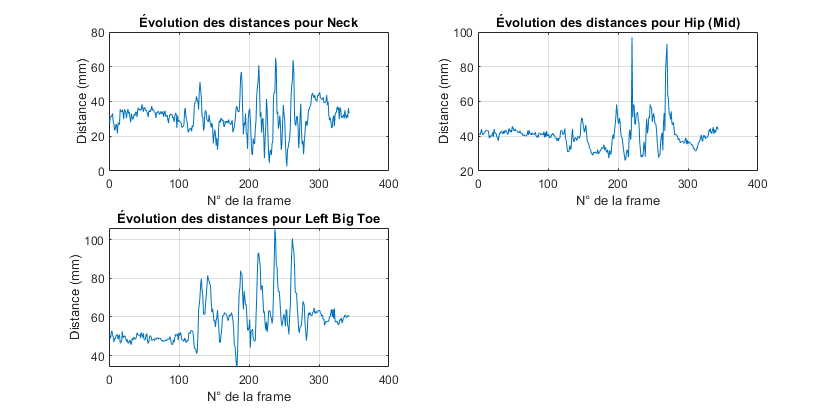
\includegraphics[width=\textwidth]{assets/Capture d'écran process/TX_ViconVSMocapIA/evolution_distance_Mocap17.png}
        \caption{Évolution de la distance}
    \end{figure}
    \begin{figure}[H]
        \centering
        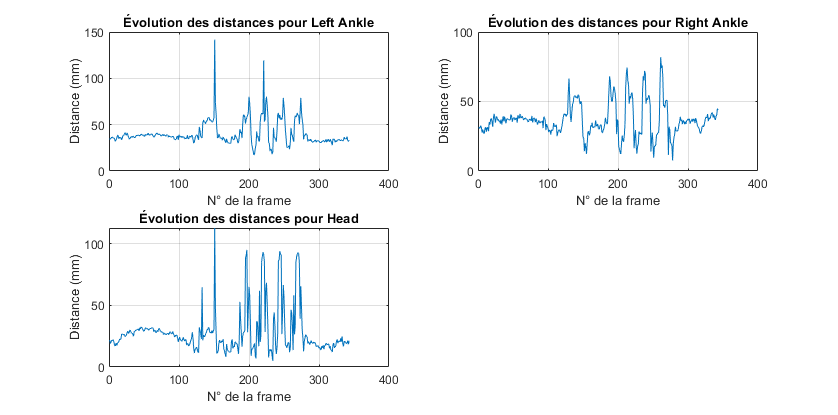
\includegraphics[width=\textwidth]{assets/Capture d'écran process/TX_ViconVSMocapIA/evolution_distance_Mocap2.png}
        \caption{Évolution de la distance}
    \end{figure}
    \begin{figure}[H]
        \centering
        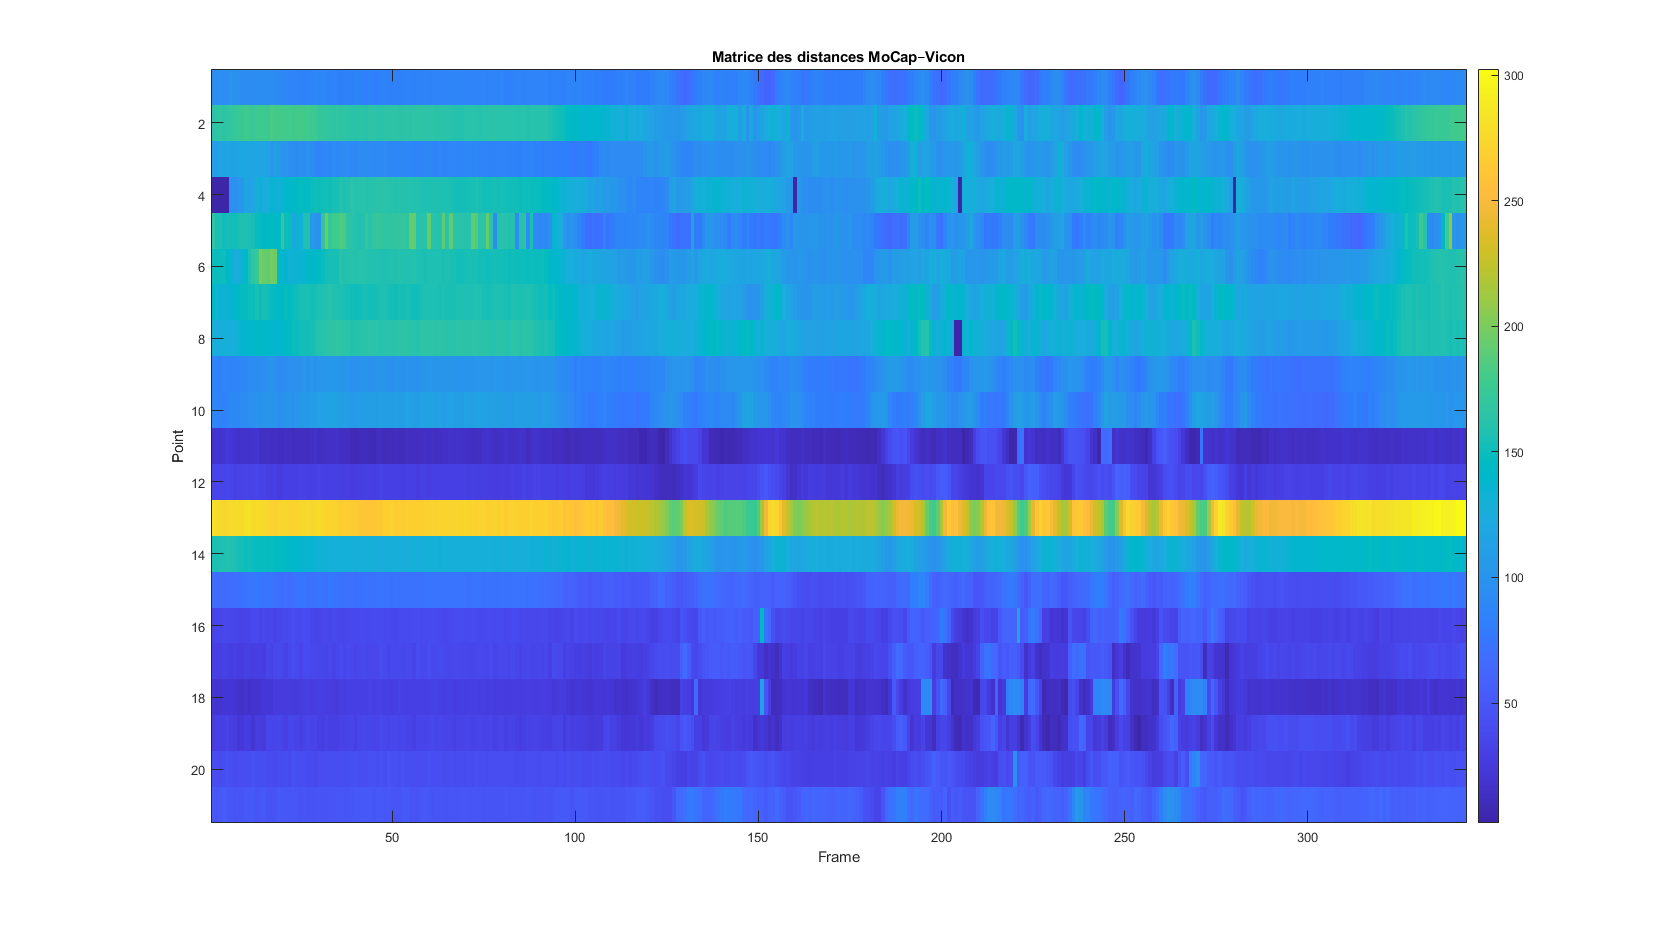
\includegraphics[width=\textwidth]{assets/Capture d'écran process/TX_ViconVSMocapIA/matrice_distances_result.png}
        \caption{Matrice des distances sur l'ensemble du mouvement entre chaque marqueur Vicon et MoCapIA}
    \end{figure}
    \begin{figure}[H]
        \centering
        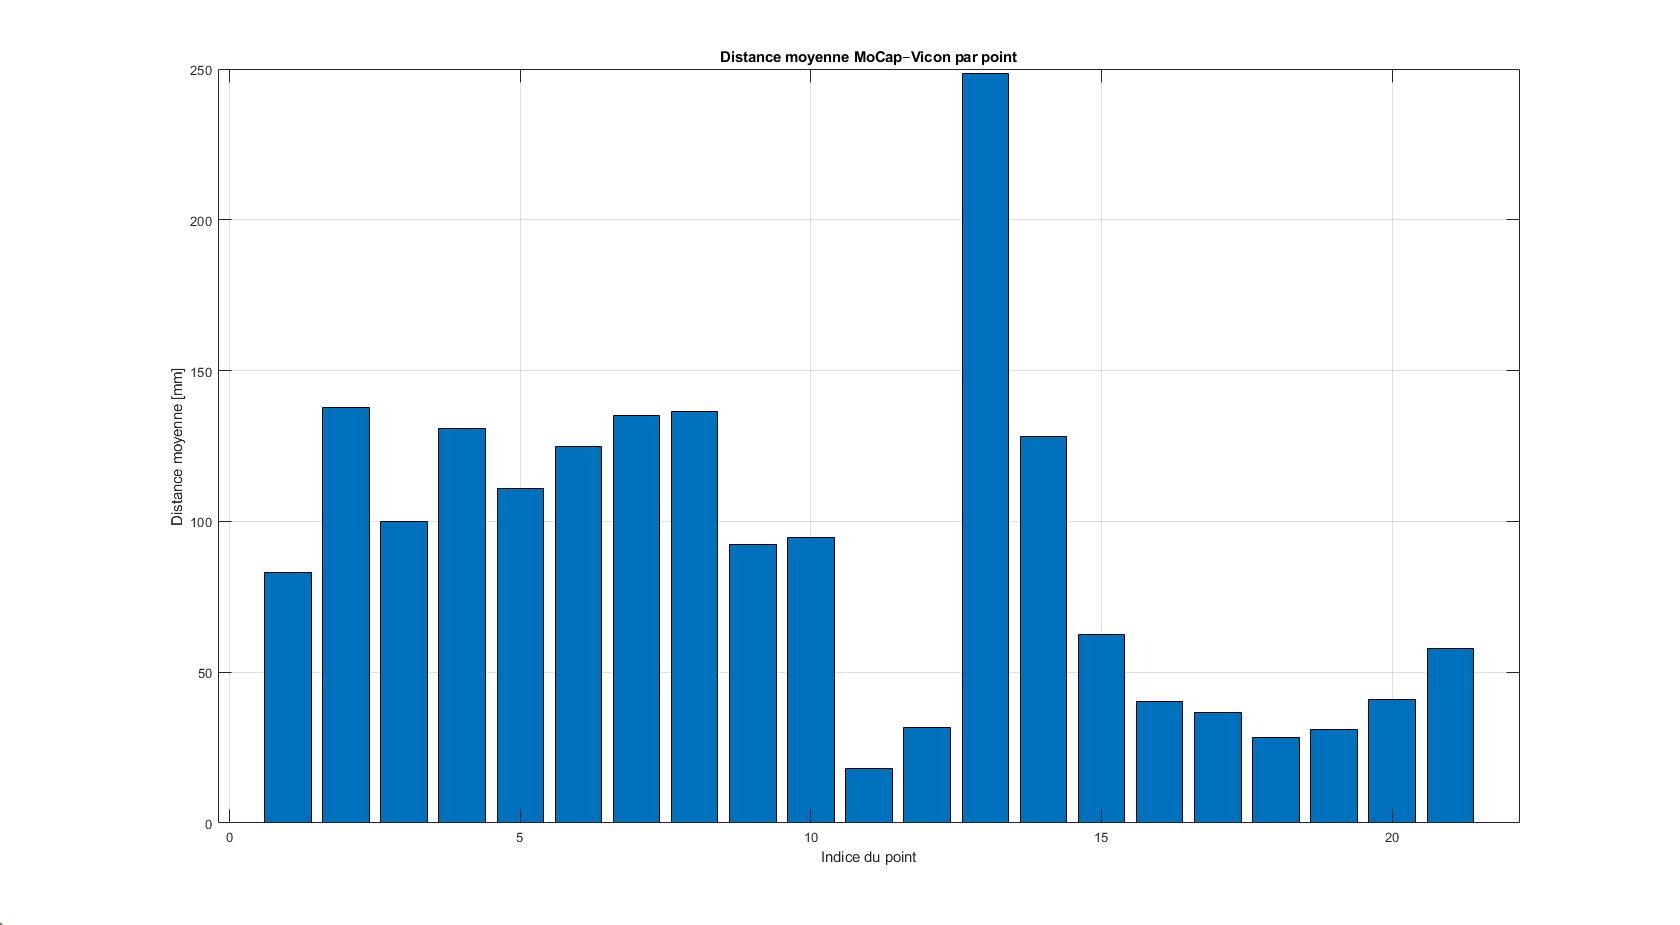
\includegraphics[width=\textwidth]{assets/Capture d'écran process/TX_ViconVSMocapIA/mean_distance.png}
        \caption{Distance moyenne entre chaque marqueur Vicon et MoCapIA}
    \end{figure}
    \begin{figure}[H]
        \centering
        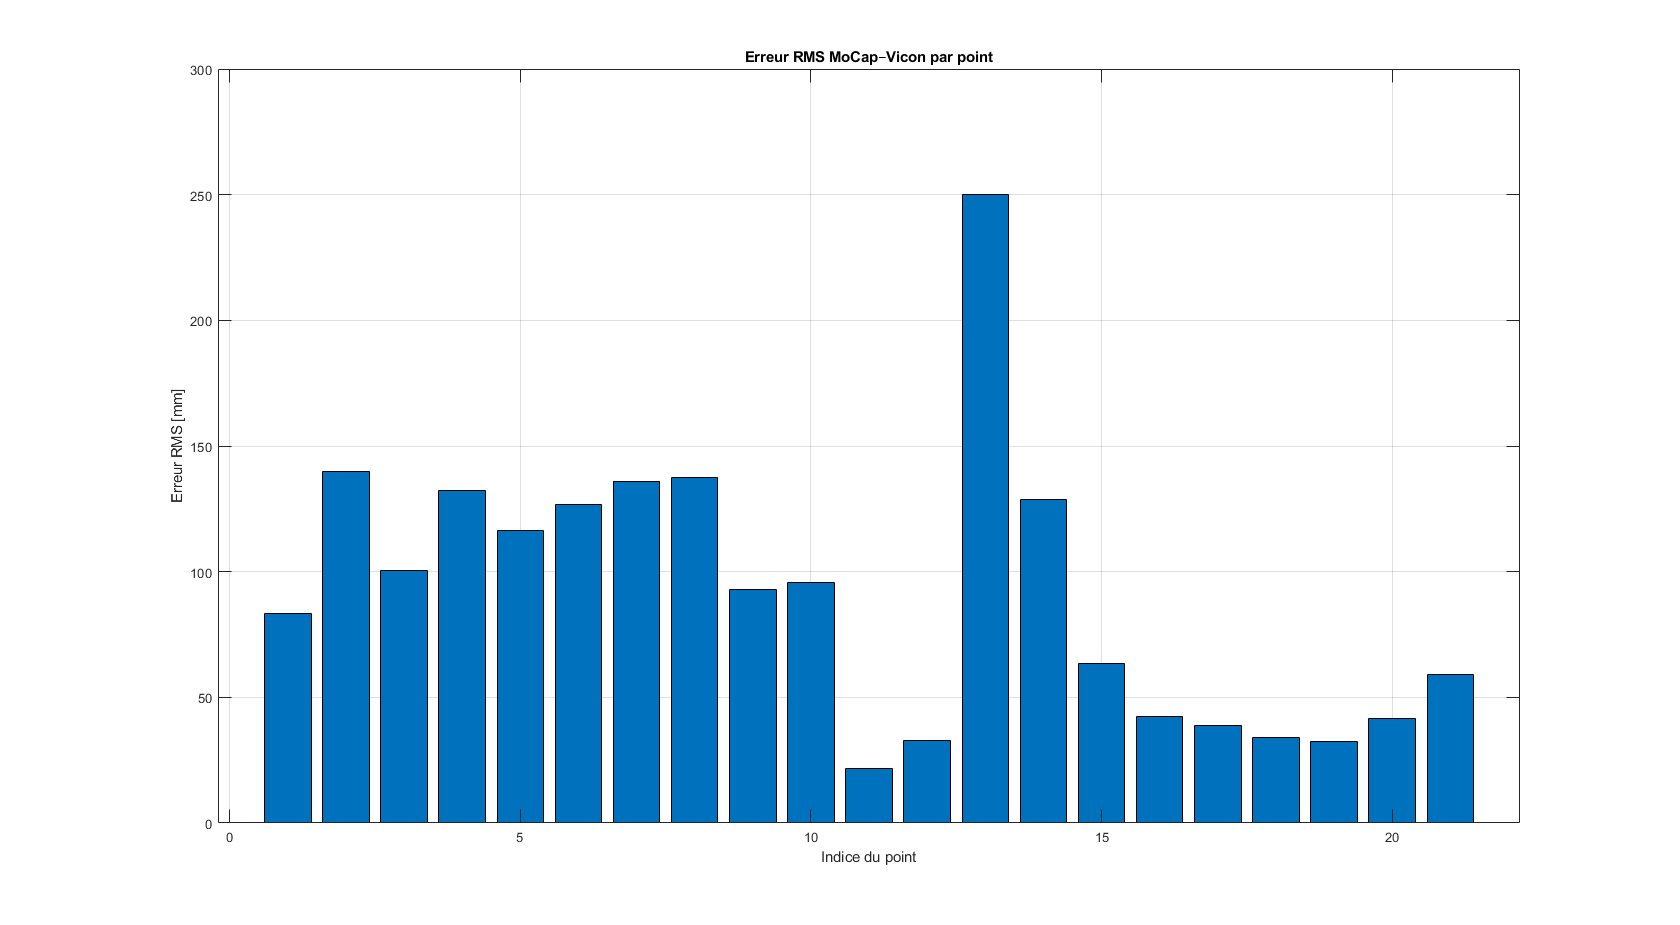
\includegraphics[width=\textwidth]{assets/Capture d'écran process/TX_ViconVSMocapIA/RMS_result.png}
        \caption{RMS des distances entre chaque marqueur Vicon et MoCapIA}
    \end{figure}

\section{Annexe 3 - résultat des autres filtres}
\label{Annexfiltres}

    Les filtres Kalman, LOESS, GCV Spline, Gaussien et Butterworth Speed ont également été testés sur les données 3D issues de MoCapIA. Les résultats, pas assez convaincant pour le filtrage d'un signal biomécanique, sont présentés dans les figures \ref{fig:kalman_result}, \ref{fig:loess_result}, \ref{fig:gcv_result}, \ref{fig:gaussian_result} et \ref{fig:butterworth_speed_result}.
    \begin{figure}[H]
        \centering
        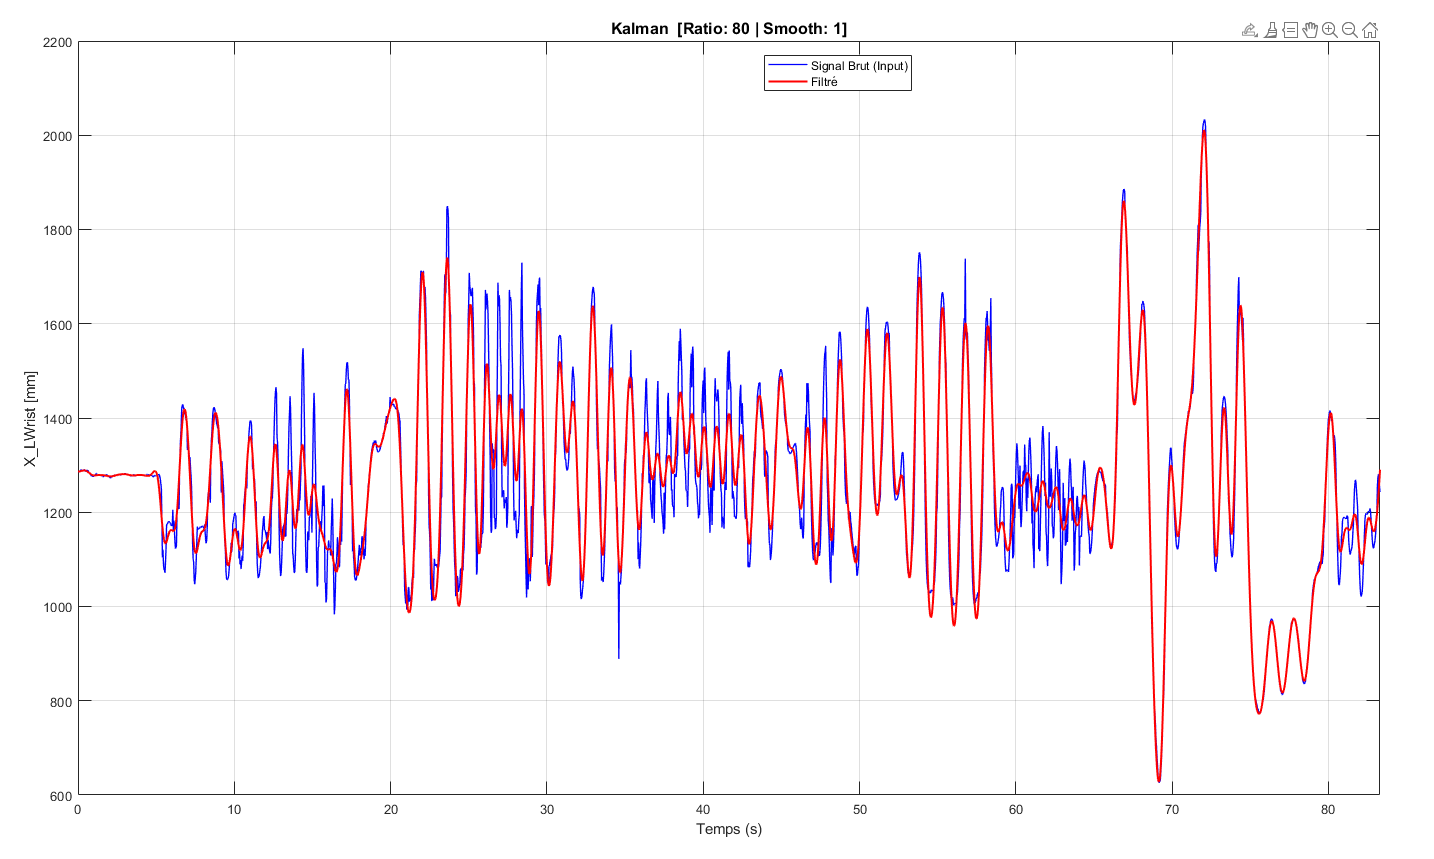
\includegraphics[width=\textwidth]{assets/Capture d'écran process/Tests Filtres 3D/valid/kalman.png}
        \caption{Résultat du filtre de Kalman avec un ratio de confiance de $150$}
        \label{fig:kalman_result}
    \end{figure}
    \begin{figure}[H]
        \centering
        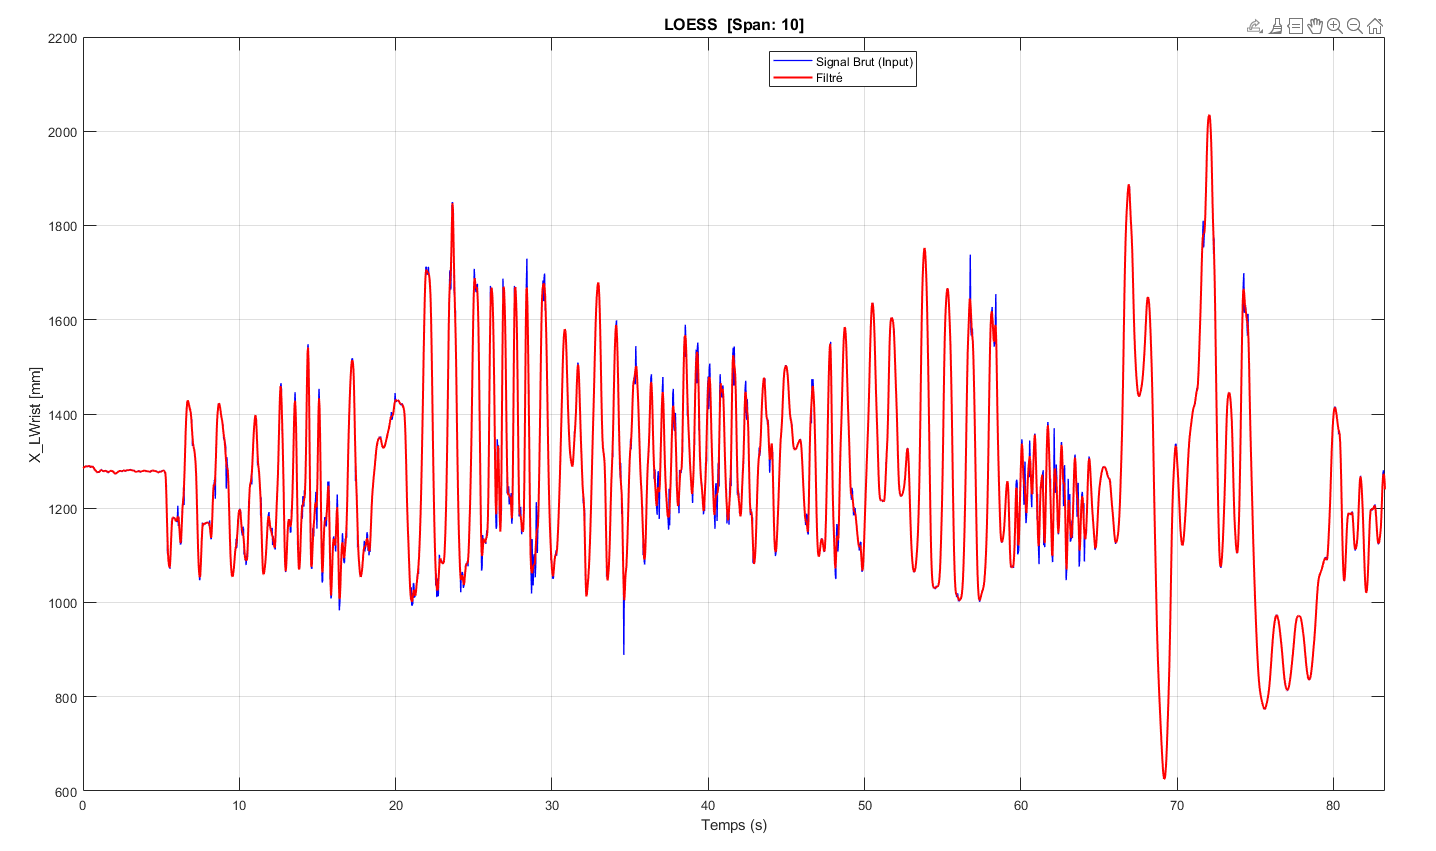
\includegraphics[width=\textwidth]{assets/Capture d'écran process/Tests Filtres 3D/valid/loess.png}
        \caption{Résultat du filtre LOESS avec un paramètre de lissage de $10$ valeurs}
        \label{fig:loess_result}
    \end{figure}
    \begin{figure}[H]
        \centering
        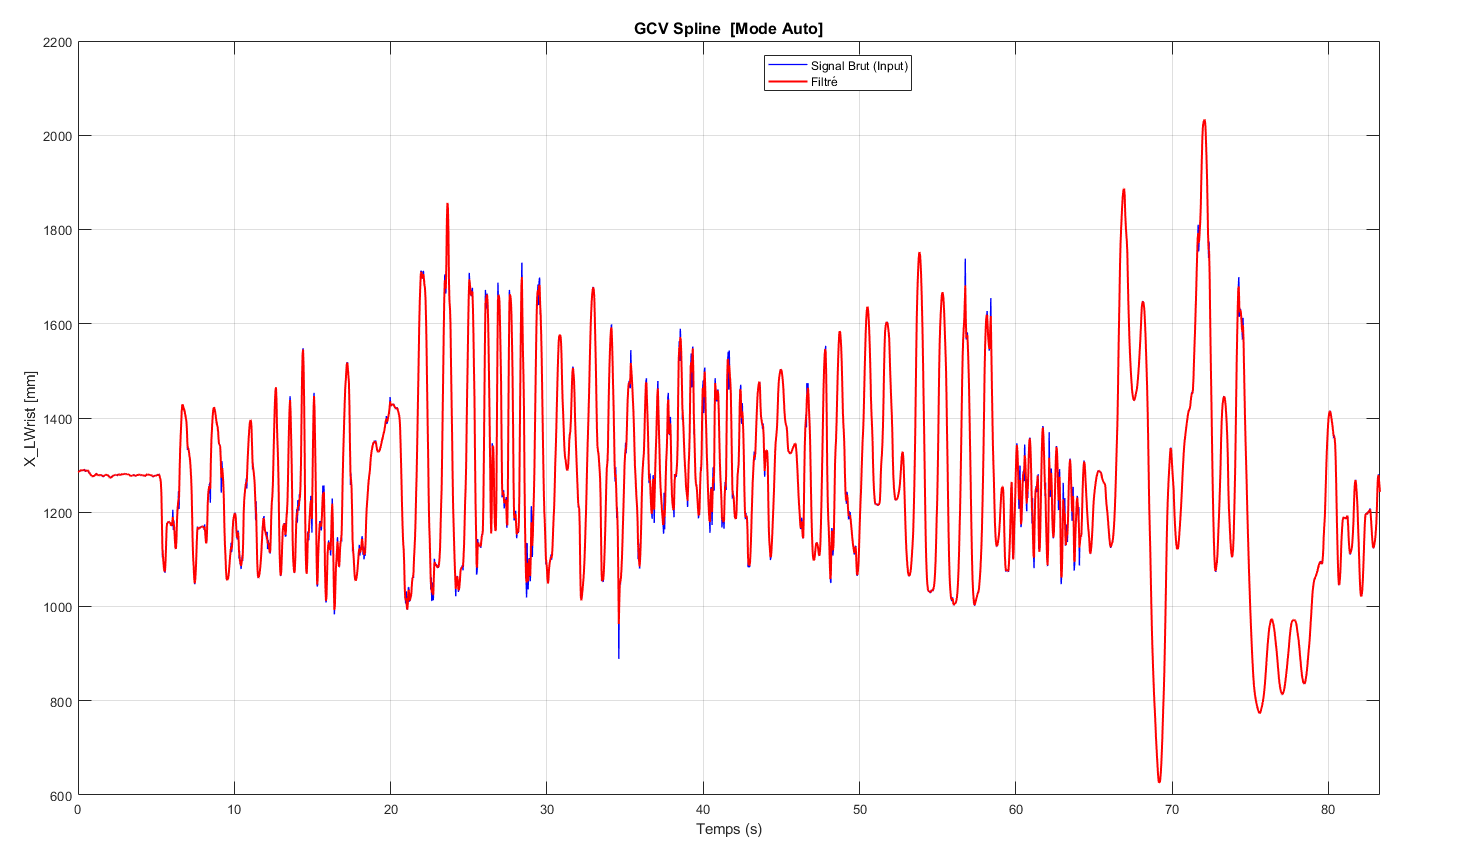
\includegraphics[width=\textwidth]{assets/Capture d'écran process/Tests Filtres 3D/valid/gcv_spline.png}
        \caption{Résultat du filtre GCV Spline}
        \label{fig:gcv_result}
    \end{figure}
    \begin{figure}[H]
        \centering
        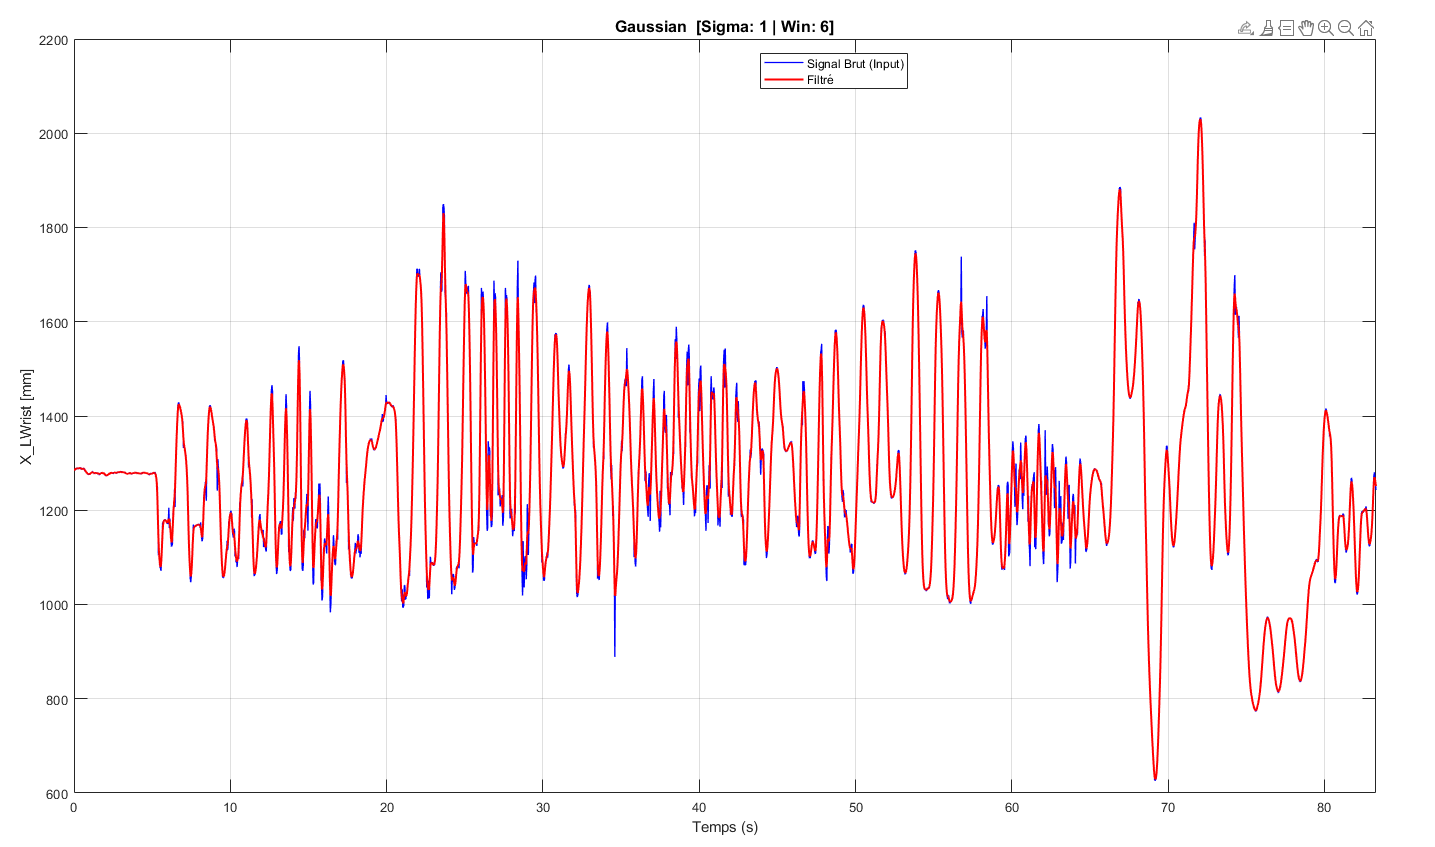
\includegraphics[width=\textwidth]{assets/Capture d'écran process/Tests Filtres 3D/valid/gaussian.png}
        \caption{Résultat du filtre Gaussien avec $sigma = 1$}
        \label{fig:gaussian_result}
    \end{figure}
    \begin{figure}[H]
        \centering
        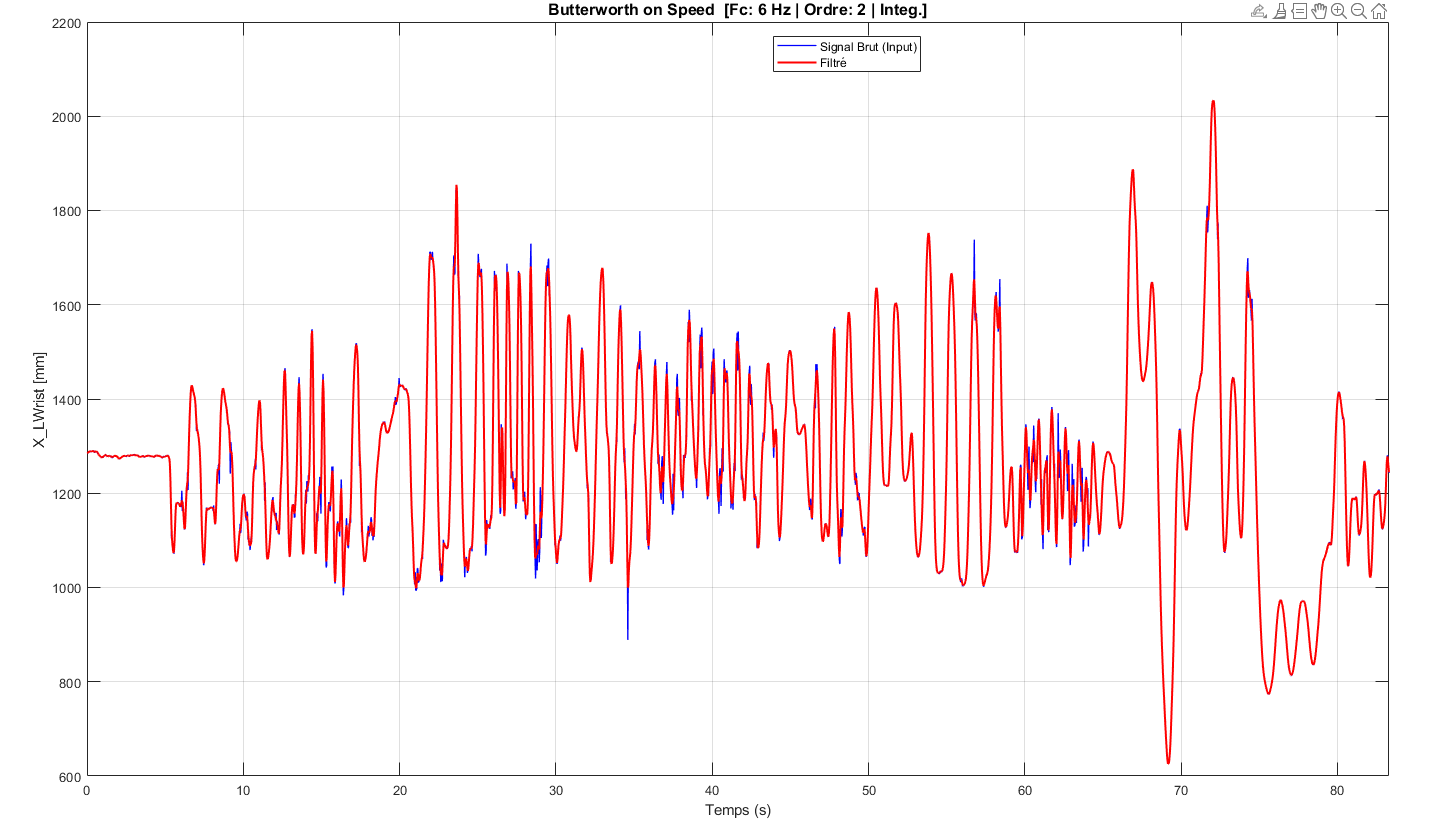
\includegraphics[width=\textwidth]{assets/Capture d'écran process/Tests Filtres 3D/valid/butterworth_speed.png}
        \caption{Résultat du filtre Butterworth Speed d'ordre 2 avec une fréquence de coupure de $6Hz$}
        \label{fig:butterworth_speed_result}
    \end{figure}

    \section{Annexe 4 - Analyse Bland-Altman de Vicon, SAM3D et MoCapIA}
    \label{AnnexBlandAltmanSAM3D}
        \begin{figure}[H]
            \centering
            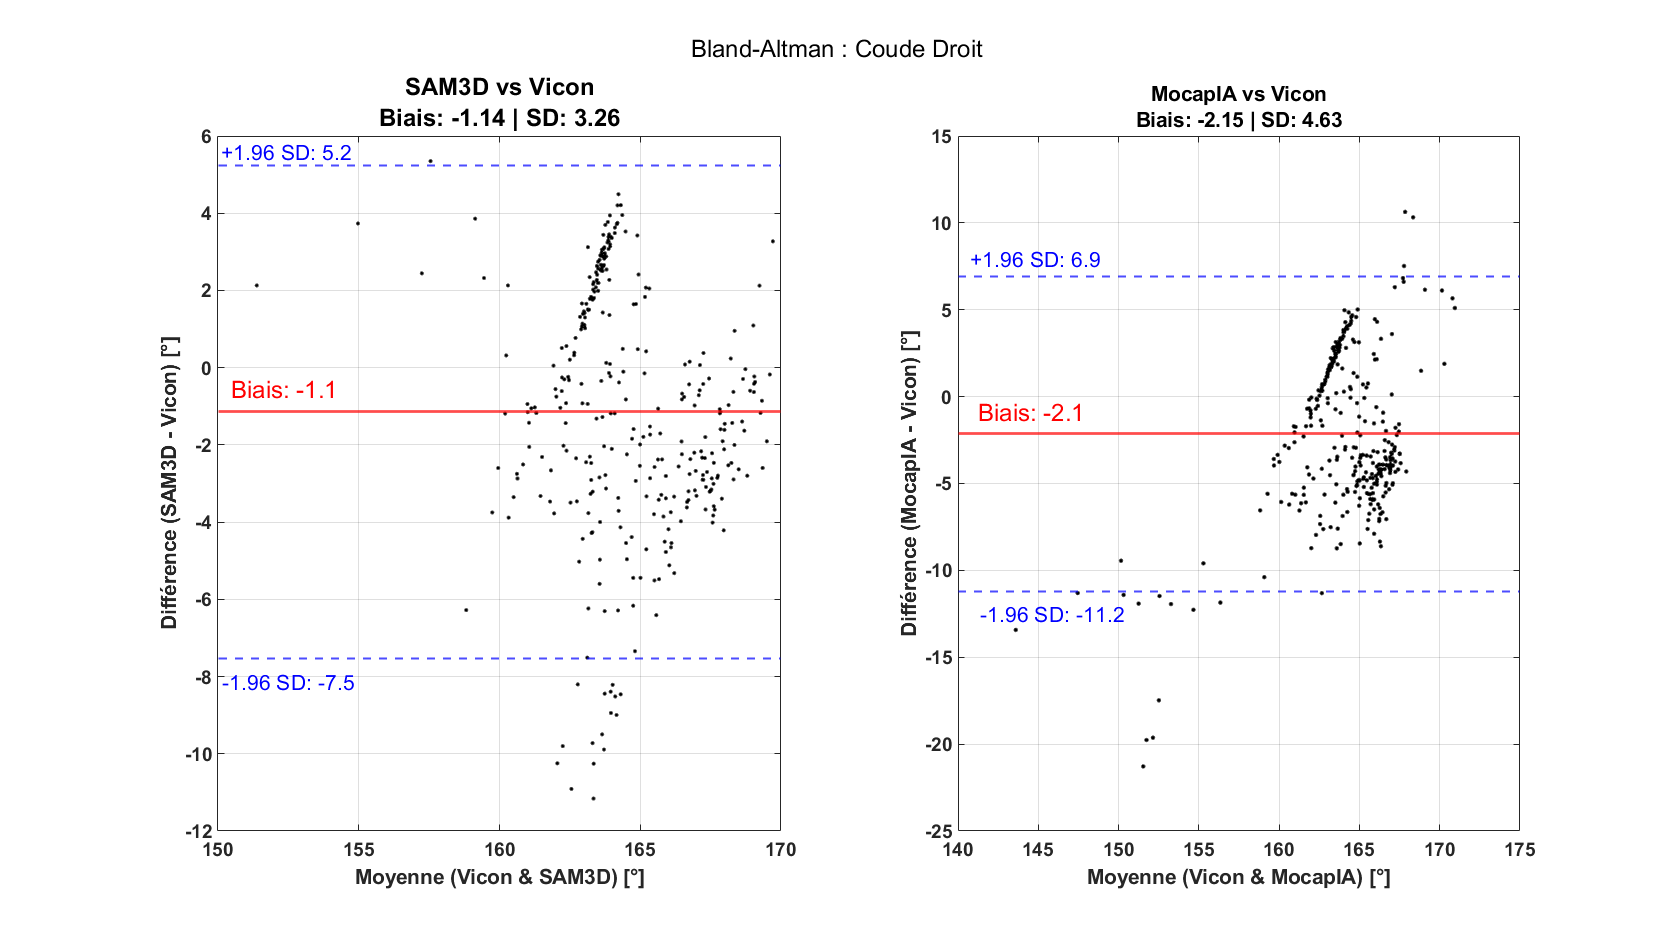
\includegraphics[width=\textwidth]{assets/Capture d'écran process/Vicon vs SAM3D vs MoCapIA/BlandAltman_Vicon_Mocap_sam3D_CoudeD.png}
            \caption{Analyse Bland-Altman entre Vicon, SAM 3D Body et MoCapIA pour le coude droit}
            \label{fig:bland_altman_vms1}
        \end{figure}
        \begin{figure}[H]
            \centering
            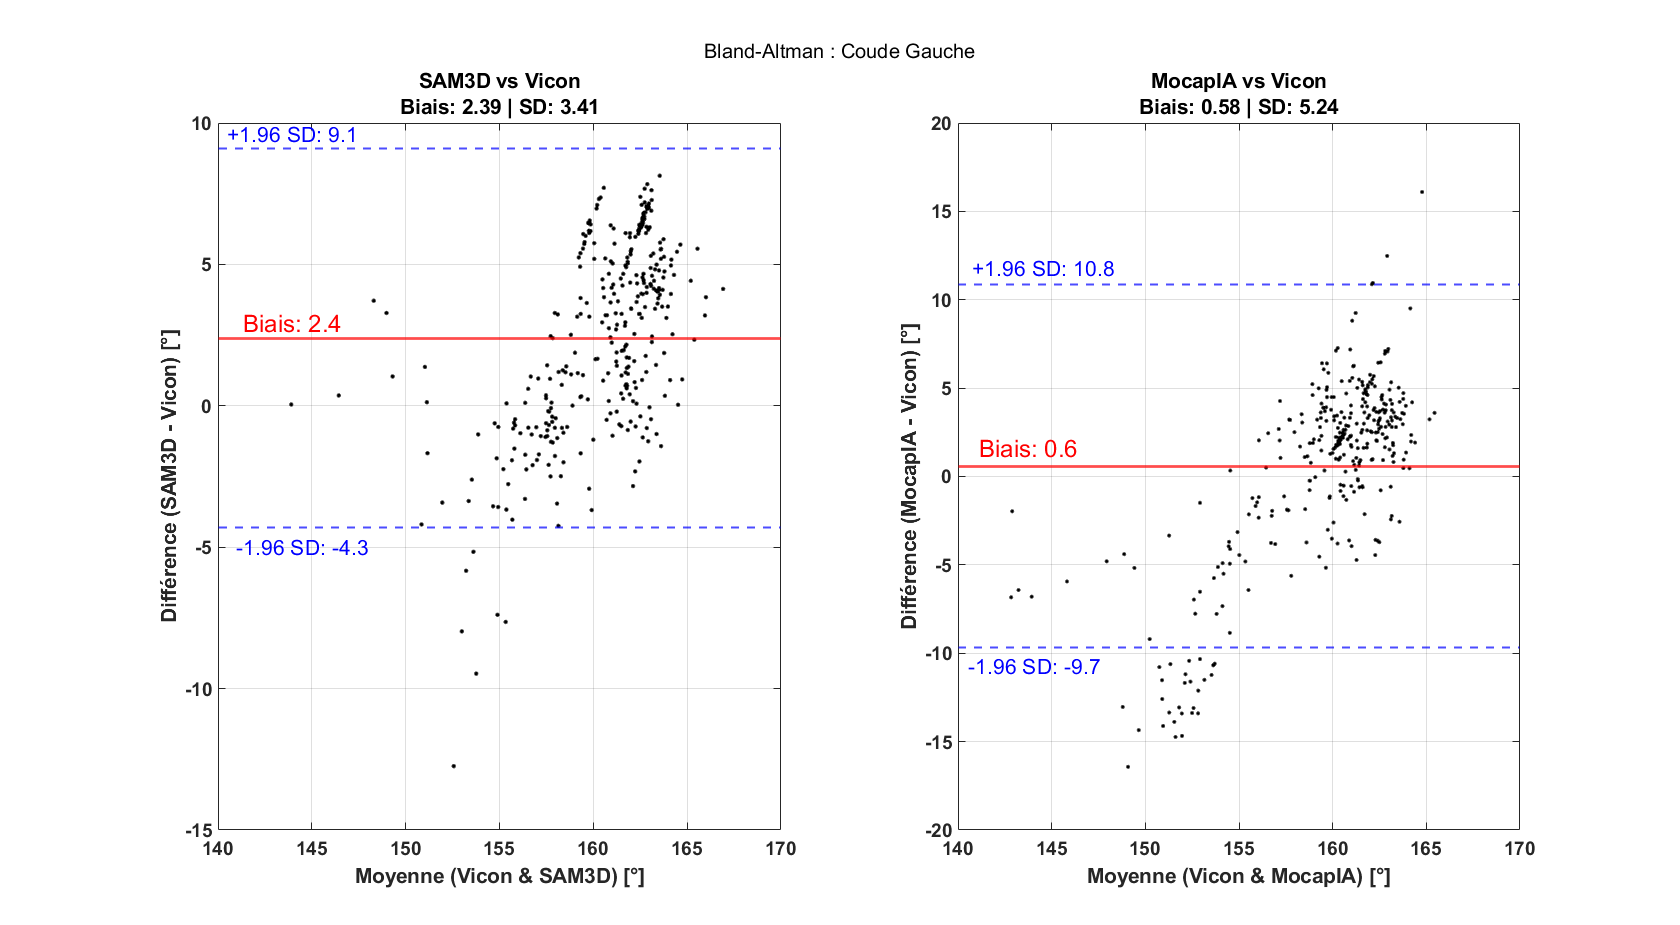
\includegraphics[width=\textwidth]{assets/Capture d'écran process/Vicon vs SAM3D vs MoCapIA/BlandAltman_Vicon_Mocap_sam3D_coudeG.png}
            \caption{Analyse Bland-Altman entre Vicon, SAM 3D Body et MoCapIA pour le coude gauche}
            \label{fig:bland_altman_vms2}
        \end{figure}
        \begin{figure}[H]
            \centering
            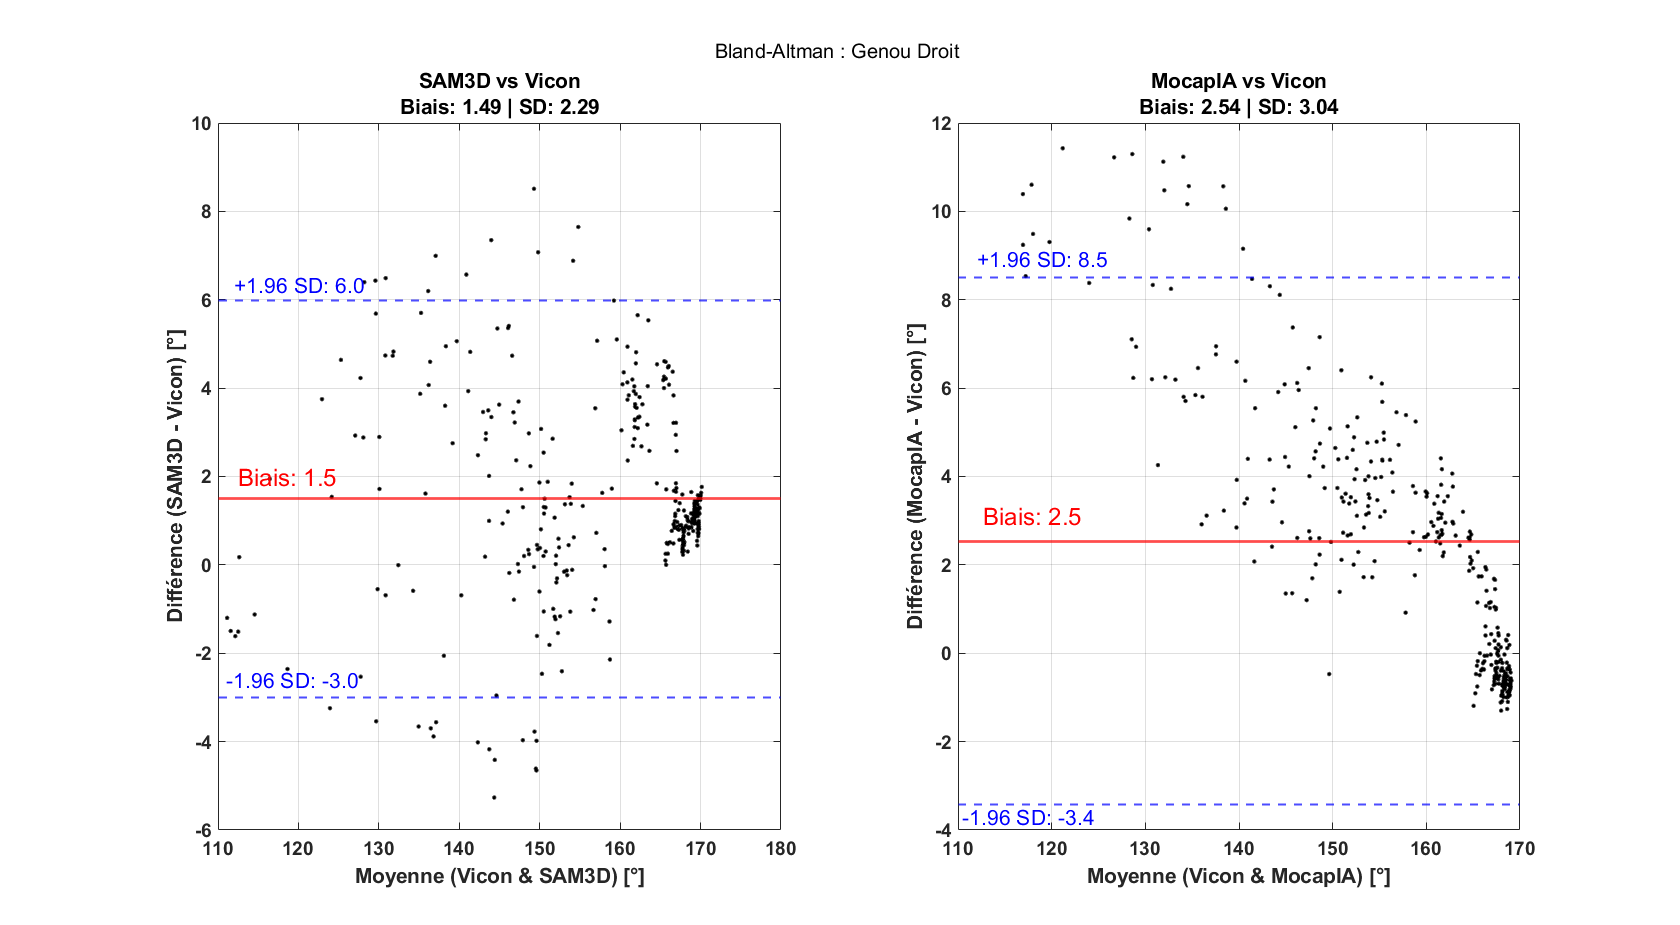
\includegraphics[width=\textwidth]{assets/Capture d'écran process/Vicon vs SAM3D vs MoCapIA/BlandAltman_Vicon_Mocap_sam3D_genouD.png}
            \caption{Analyse Bland-Altman entre Vicon, SAM 3D Body et MoCapIA pour le genou droit}
            \label{fig:bland_altman_vms3}
        \end{figure}
            